\chapter{RADAMS: Data provenance} % (fold)
\label{cha:radams_data_provenance}
	
	In this section, we will deal with the data provenance part of
	the RADAMS. This sub data model provides support for the
	description of how data have been generated.
	
	 As we saw in the RADAMS overview
	---chapter~\ref{cha:radams}---, we have divided data provenance
	in three parts:
	
	\begin{description}
		\item[Instrumental] Has to do with the instrumental setup,
		i.e., the configuration of all observation elements between
		the original photon source and the photon detection
		equipment.
		
		 \item[Environmental] Has to do with the elements in the
		path of the photon source which cannot be controlled by the
		instrumental setup, but that nonetheless affect the photon
		collection (i.e., by causing turbulence, changing the
		refraction index, or absorbing photons). We will register
		measurable environmental parameters in order to estimate
		possible effects and/or defects in the detections.
		
		 \item[Processing] Once raw data are recorded, many
		different processing steps need to be performed in order to
		provide science-ready data, or as it is sometimes said,
		data are provided with the instrument signature removed as
		much as possible. Processing Provenance records the
		different processes and their inputs performed in order to
		achieve the result being offered by the archive.
	\end{description}
	
	We will study each one in detail in the following sections.
	
	\section{Instrumental provenance} % (fold)
	\label{sec:instrumental_provenance}
		
		Figure \ref{figProvenanceInstrument} shows the classes
		associated with the instrumental configuration for the
		observation.

		\begin{figure}[tbp]
		\begin{center}
		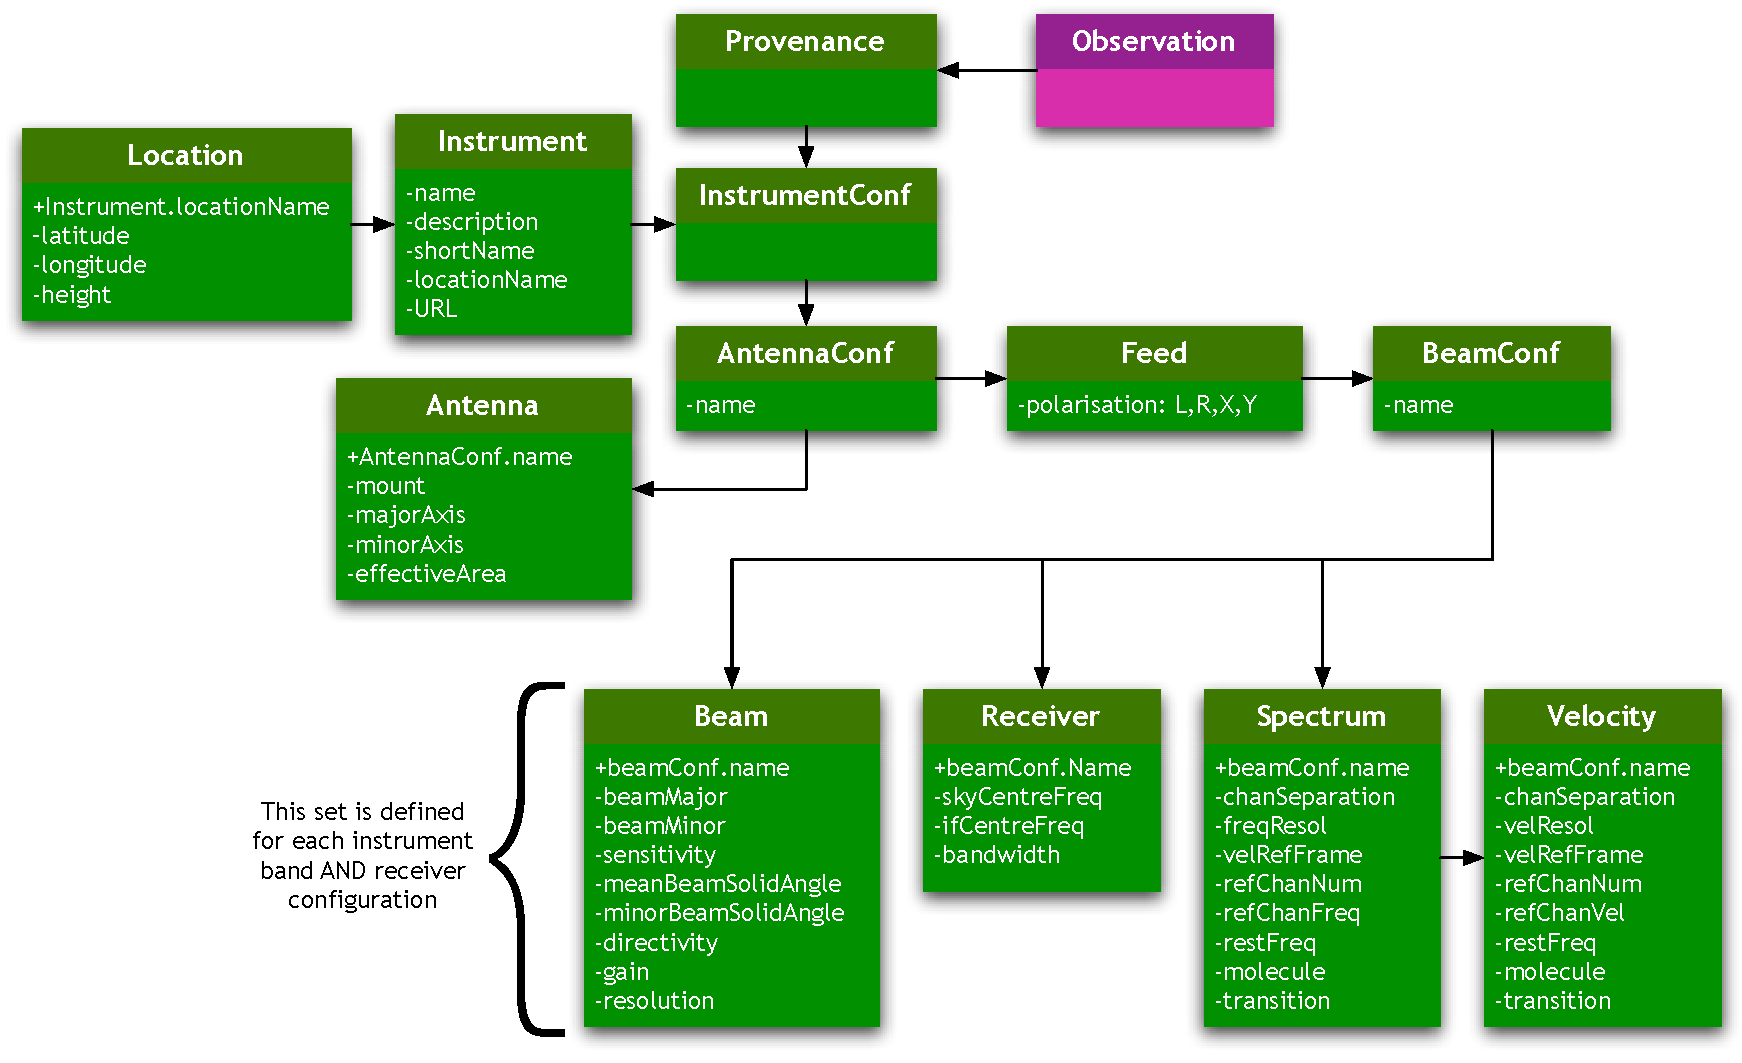
\includegraphics[width=\columnwidth]
		{fig/Provenance-Instrument-DM}
		\end{center}
		\caption[Provenance.Instrument data model]
		{Provenance.Instrument data model.}
		\label{figProvenanceInstrument}
		\end{figure}
		
		\begin{description}
			\item[InstrumentConf] Each observation is associated to
			a particular instrumental configuration, which results
			from the particular configuration of the instrument +
			antenna + feed system. InstrumentConf instances group
			those settings.
			
			 \item[Instrument] Instances of this class specify the
			instrument configuration, as used for the observation.
			
			 \item[Instrument.Location] This is an instance of a
			Location class, used for specifying the location for
			the instrument.
			
			 \item[AntennaConf] In the same way InstrumentConf
			allows the grouping for all the instrumental settings,
			AntennaConf instances group together Antenna and Feed
			info (regarding polarisation), plus the BeamConf ---another
			aggregator class---. Several AntennaConf instances
			can provide information for different antennas and
			feeds. Each possible antenna configuration will be
			labelled by a name.
			
			 \item[Antenna] Instances of this class specify the
			general properties for each given antenna. We will also
			use these instances to specify the type of scan being
			performed on the source from a controlled vocabulary.
			
			 \item[Feed] Instances of this class ---one or more per
			AntennaConf--- specify each of the feed horns used for
			the observation, and their corresponding polarisation
			from a controlled vocabulary: \texttt{L}, \texttt{R},
			\texttt{X}, \texttt{Y}. We cannot make use of the
			Stokes polarisation parameters, as they cannot be
			directly measured via the feed configuration: instead,
			they have to derived by means of data processing steps.
			
			 \item[BeamConf] This class is used to group antennas,
			feeds, and beams. The relationship between BeamConf and
			Feed instances allows the specification of different
			beams, formed by the combination of different feeds. In
			a single-dish single-feed configuration, there is only
			one beam associated to a given receiver. We can also
			use this association for a single-dish, multiple-feed
			configuration where each feed goes to a different
			receiver.
			
			 \item[Beam] Metadata for this class specifies the
			actual beam for the telescope, associated to a given
			spectral band.
			
			 \item[Receiver] This metadata are used to describe the
			most relevant properties of the receiver, such as
			receiver type, intermediate frequency ---in the case of
			heterodyne stages---, et cetera.
			
			 \item[Spectrum] In case of spectroscopic observations,
			the spectral analyser that has been used is specified
			by instances of this class.
			
			 \item[Velocities] This class mirrors the Spectrum
			class, and is preferred for those cases where
			velocities are used, instead of frequency.
		\end{description}

		\begin{table}
		\caption[Provenance instrument metadata]
		{Provenance instrument metadata.}
		\begin{smallertabular}{p{2.15 cm}p{1.5cm}p{2.25cm}p{5.35cm}}
			& \textbf{FITS} & & \\ \textbf{Attribute} &
            \textbf{Keyword} & \textbf{UCD} & \textbf{Description}\\
            \midrule name & \texttt{INSTRUME} & \texttt{meta.id; instr;
            meta.main} & Instrument name.\\ \addlinespace description &
            \texttt{assign} & \texttt{meta.note; meta.main} &
            Instrument description.\\ \addlinespace shortName &
            \texttt{assign} & \texttt{instr; meta.id} & Short name for
            the instrument.\\ \addlinespace locationName &
            \texttt{assign} & \texttt{instr; pos; meta.id} &
            Localisation of the instrument.\\ \addlinespace URL &
            \texttt{COMMENT} & \texttt{instr; meta.ref.url} & URL for
            the instrument (website for the instrument, documentation,
            or any other type of instrument description).\\
            \addlinespace
		\end{smallertabular}
		\label{tabProvenanceInstrument}
		\end{table}

		\begin{table}
		\caption[Instrument location metadata]
		{Instrument location metadata.}
		\begin{smallertabular}{p{2 cm}p{1.5cm}p{3.2cm}p{4.55cm}}
					& \textbf{FITS} & & \\ \textbf{Attribute} &
		            \textbf{Keyword} & \textbf{UCD} & \textbf{Description}\\
		            \midrule locationName & \texttt{assign} &
		            \texttt{instr; pos; meta.id} & Name of a particular
		            instrument location.\\ \addlinespace latitude & \texttt{SITELAT}
		            & \texttt{instr; pos.earth.lat} & Instrument location
		            latitude.\\ \addlinespace longitude & \texttt{SITELONG} &
		            \texttt{instr; pos.earth.lon} & Instrument location
		            longitude.\\ \addlinespace altitude & \texttt{SITEELEV} &
		            \texttt{instr; pos.earth.altitude} & Instrument location
		            altitude.\\ \addlinespace
		\end{smallertabular}
		\label{tabProvenanceInstrLocation}
		\end{table}

		\begin{table}
		\caption[Antenna configuration metadata]
		{Antenna configuration metadata.}
		\begin{smallertabular}{p{2 cm}p{1.5cm}p{3.2cm}p{4.55cm}}
					& \textbf{FITS} & & \\ \textbf{Attribute} &
		            \textbf{Keyword} & \textbf{UCD} & \textbf{Description}\\
		            \midrule name & \texttt{assign} & \texttt{instr.telescope;
		            meta.title; meta.id} & Name of the particular antenna.\\
		            \addlinespace scanType & \texttt{assign} &
		            \texttt{instr.setup; meta.code} & Type of scan being
		            performed by this antenna, from a limited vocabulary
		            (suggested by the RDM \cite{LamPow0310IVOA}):
		            \texttt{beam\-Switch}, \texttt{cal}, \texttt{cross},
		            \texttt{dop\-pler\-Track}, \texttt{dwell},
		            \texttt{fo\-cus}, \texttt{fre\-quen\-cy\-Switch},
		            \texttt{hol\-og\-ra\-phy}, \texttt{mo\-sa\-ic},
		            \texttt{on\-Off}, \texttt{on\-The\-Fly}, \texttt{point},
		            \texttt{pos\-i\-tion\-Switch}, \texttt{pul\-sar},
		            \texttt{ras\-ter}, \texttt{sky\-Dip}, \texttt{tiedArray},
		            \texttt{track}, \texttt{wob\-bler\-Switch}.\\ \addlinespace
		            mount & \texttt{assign} & \texttt{meta.note} & Mount type
		            for the telescope from a limited vocabulary:
		            \texttt{azimuthal}, \texttt{e\-qua\-to\-ri\-al},
		            \texttt{alt\-az\-i\-muth\-al}, \texttt{dobson},
		            \texttt{german e\-qua\-to\-ri\-al}.\\ \addlinespace
		            majorAxis & \texttt{assign} & \texttt{instr;
		            phys.size.smajAxis} & Major axis dimensions.\\
		            \addlinespace minorAxis & \texttt{assign} & \texttt{inst;
		            phys.size.sminAxis} & Minor axis dimensions.\\
		            \addlinespace effectiveArea & \texttt{assign} &
		            \texttt{instr; phys.area} & Effective instrument area.\\
		            \addlinespace
		\end{smallertabular}
		\label{tabProvenanceInstrAntenna}
		\end{table}

		\begin{table}
		\caption[Feed configuration metadata]{Feed configuration metadata.}
		\begin{smallertabular}{p{2 cm}p{1.5cm}p{3.2cm}p{4.55cm}}
					& \textbf{FITS} & & \\ \textbf{Attribute} &
		            \textbf{Keyword} & \textbf{UCD} & \textbf{Description}\\
		            \midrule polarisation & \texttt{STOKES} &
		            \texttt{pos.posAng; phys.polarization; meta.code} &
		            Polarisation value from a controlled vocabulary:
		            \texttt{L}, \texttt{R}, \texttt{X}, \texttt{Y}\\
		            \addlinespace
		\end{smallertabular}
		\label{tabProvenanceInstrFeed}
		\end{table}

		\begin{table}
		\begin{minipage}{\linewidth}
		\caption[Beam configuration metadata]{Beam configuration metadata.}
		\begin{smallertabular}{p{3 cm}p{1.5cm}p{3.35cm}p{3.40cm}}
					& \textbf{FITS} & & \\ \textbf{Attribute} &
		            \textbf{Keyword} & \textbf{UCD} & \textbf{Description}\\
		            \midrule beamMajor & \texttt{BMAJ/HPBW} &
		            \texttt{instr.beam; phys.size.smajAxis} & Major axis HPBW
		            of the main lobe of the beam.\\ \addlinespace beamMinor &
		            \texttt{BMIN/HPBW} & \texttt{instr.beam;
		            phys.size.sminAxis} & Minor axis HPBW of the main lobe of
		            the beam.\\ \addlinespace sensitivity & \texttt{BEAMEFF} &
		            \texttt{instr.beam; instr.sensitivity} & Beam average
		            sensitivity.\\ \addlinespace mainBeamSolidAngle &
		            \texttt{assign} & \texttt{instr.beam; pos.posAng;
		            meta.main} & Main lobe’s beam solid angle.\\ \addlinespace
		            totalBeamSolidAngle & \texttt{assign} &
		            \texttt{instr.beam; pos.posAng; stat.max} & Total beam
		            solid angle, including secondary lobes.\\ \addlinespace
		            directivity & \texttt{assign} & \texttt{instr.beam;
		            instr.setup; arith.factor} & Directivity percentage.\\
		            \addlinespace gain & \texttt{ANTGAIN} & \texttt{instr.beam;
		            instr.setup; arith.factor} & Beam gain\footnote{We still
		            have to clarify if the gain attribute is related to the
		            directivity concept or not, and if it is related with the
		            receiving stages or not.}.\\ \addlinespace
		\end{smallertabular}
		\label{tabProvenanceInstrBeam}
		\end{minipage}
		\end{table}

		\begin{table}
		\caption[Receiver metadata]{Receiver metadata.}
		\begin{smallertabular}{p{2.15 cm}p{1.5cm}p{2.35cm}p{5.25cm}}
					& \textbf{FITS} & & \\ \textbf{Attribute} &
		            \textbf{Keyword} & \textbf{UCD} & \textbf{Description}\\
		            \midrule type & \texttt{BACKEND} &
		            \texttt{instr.setup; meta.note} & Receiver type (HEMT,
		            Bolo\-meter, SIS,
					et cetera).\\ \addlinespace skyCentreFreq & \texttt{assign} &
		            \texttt{src; em.radio; em.freq} & Antenna tuning
		            frequency.\\ \addlinespace IFCentreFreq & \texttt{assign} &
		            \texttt{instr.setup; em.freq} & Heterodyne receiver
		            intermediate frequency (or list of frequencies).\\ \addlinespace
		            bandwidth & \texttt{BANDWID} & \texttt{instr.bandwidth} &
		            Filter-bank total bandwidth.\\ \addlinespace
		\end{smallertabular}
		\label{tabProvenanceInstrReceiver}
		\end{table}

		\begin{table}
		\begin{minipage}{\linewidth}
		\caption[Spectrum metadata]
		{
			Spectrum metadata. It might be necessary to change the
		    \texttt{MOLECULE} and \texttt{TRANSITI} keywords by
		    \texttt{LINE}, for better CLASS compatibility.
		}
		\begin{smallertabular}{p{2 cm}p{1.5cm}p{3.4cm}p{4.35cm}}
					& \textbf{FITS} & & \\ \textbf{Attribute} &
		            \textbf{Keyword} & \textbf{UCD} & \textbf{Description}\\
		            \midrule numChannels & \texttt{NAXISn} &
		            \texttt{spect; em.freq; meta.number} & Number of spectral
		            channels.\\ \addlinespace chanSeparation\footnote{There is a
		            certain redundancy between the
		            Provenance.Spectrum.chanSeparation attribute and the
		            Coverage.Spectral.Resolution attributes.} &
		            \texttt{assign} & \texttt{spect; em.freq} & Mean channel
		            separation (in frequency units), or channel frequency
		            separation array.\\ \addlinespace freqResolution &
		            \texttt{FREQRES} & \texttt{spect.resolution; em.freq} &
		            Frequency resolution.\\ \addlinespace refChanNum &
		            \texttt{assign} & \texttt{spect; em.freq; meta.number;
		            meta.ref} & Spectral reference channel.\\ \addlinespace
		            refChanFreq & \texttt{OBSFREQ } & \texttt{spect; em.freq;
		            meta.code; meta.ref} & Spectral reference frequency
		            (observed frequency).\\ \addlinespace restFreq & \texttt{FREQn}
		            or \texttt{RESTFREQ} & \texttt{spect.line; em.freq} &
		            Observed spectral line rest frequency.\\ \addlinespace molecule
		            & \texttt{MOLECULE}\footnote{It might be necessary to
		            change the \texttt{MOLECULE} keyword by \texttt{LINE},
		            for better CLASS compatibility.} & \texttt{spect;
		            phys.mol; meta.id} & Molecule name.\\ \addlinespace transition &
		            \texttt{TRANSITI}\footnote{It might be necessary to
		            change the \texttt{TRANSITI} keyword by \texttt{LINE},
		            for better CLASS compatibility.} & \texttt{spect;
		            phys.atmol.transition; meta.id} & Transition.\\ \addlinespace
		\end{smallertabular}
		\label{tabProvenanceInstrSpectrum}
		\end{minipage}
		\end{table}

		\begin{table}
		\begin{minipage}{\linewidth}
		\caption[Velocity metadata]{Velocity metadata.}
		\begin{smallertabular}{p{2 cm}p{1.5cm}p{3.4cm}p{4.35cm}}
				& \textbf{FITS} & & \\ \textbf{Attribute} & \textbf{Keyword} &
		        \textbf{UCD} & \textbf{Description}\\ \midrule numChannels
		        & \texttt{assign} & \texttt{spect; phys.veloc; meta.number} &
		        Number of velocity channels.\\ \addlinespace
		        chanSeparation\footnote{There is a certain redundancy between
		        the Provenance.Velocity.chanSeparation attribute and the
		        Coverage.Spectral.Resolution attributes.} & \texttt{assign} &
		        \texttt{spect; phys.veloc} & Mean channel separation (in
		        velocity units), or velocity channel separation array.\\ \addlinespace
		        velResolution & \texttt{assign} & \texttt{spect.resolution;
		        phys.veloc} & Velocity resolution.\\ \addlinespace velRefFrame &
		        \texttt{assign} & \texttt{spect; phys.veloc; pos.frame;
		        meta.id} & Identification of the reference system used for the
		        velocity.\\ \addlinespace refChanNum & \texttt{assign} &
		        \texttt{spect; phys.veloc; meta.number; meta.ref} & Velocity
		        reference channel.\\ \addlinespace refChanFreq & \texttt{assign } &
		        \texttt{spect; phys.veloc; meta.code; meta.ref} & Frequency for
		        the velocity reference channel.\\ \addlinespace restFreq &
		        \texttt{RESTFREQ} & \texttt{spect.line; em.freq} & Observed
		        spectral line rest frequency.\\ \addlinespace molecule &
		        \texttt{MOLECULE}\footnote{It might be necessary to change the
		        \texttt{MOLECULE} keyword by \texttt{LINE}, for better CLASS
		        compatibility.} & \texttt{spect; phys.mol; meta.id} & Molecule
		        name.\\ \addlinespace transition & \texttt{TRANSITI}\footnote{It might
		        be necessary to change the \texttt{TRANSITI} keyword by
		        \texttt{LINE}, for better CLASS compatibility.} &
		        \texttt{spect; phys.atmol.transition; meta.id} & Transition.\\
		        \addlinespace
		\end{smallertabular}
		\label{tabProvenanceInstrVelocity}
		\end{minipage}
		\end{table}
		
	% section instrumental_provenance (end)
	
	\section{Environmental provenance} % (fold)
	\label{sec:environmental_provenance}
		
		Environmental provenance is the part of the provenance
		dealing with ambient conditions, and as such the main class
		is called Provenance.AmbientConditions: it encompasses all
		metadata needed to specify weather conditions, air mass, 
		opacity, et cetera. Figure
		\ref{figProvenanceAmbient} shows the corresponding classes and
		their relationships.

		\begin{figure}[tbp]
		\begin{center}
		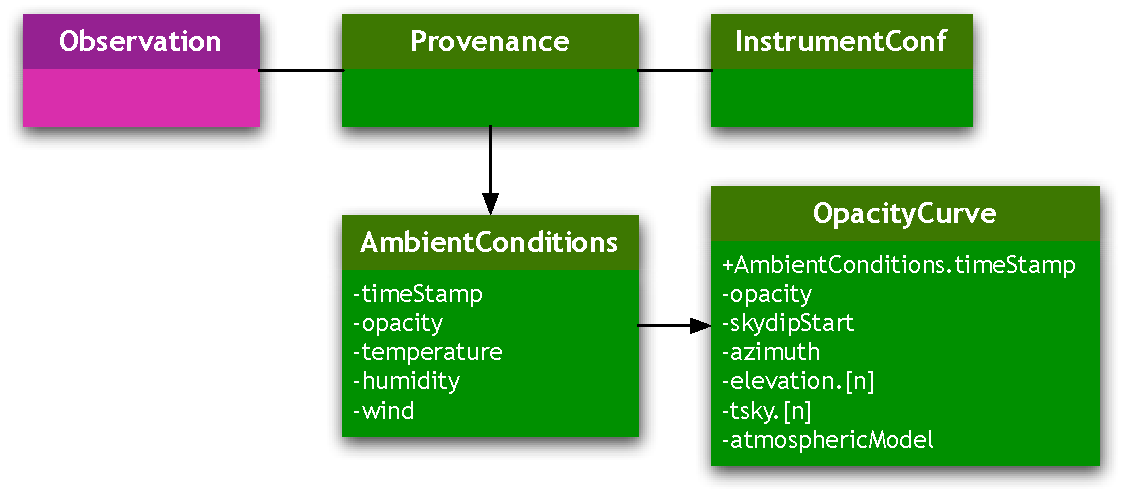
\includegraphics[width=\columnwidth]
			{fig/Provenance-AmbientConditions-DM}
		\end{center}
		\caption[Provenance.AmbientConditions data model]
			{Provenance.AmbientConditions data model.}
		\label{figProvenanceAmbient}
		\end{figure}
		
		
		\begin{description}
			\item[AmbientConditions] Holds all metadata related
			with weather conditions for the observation, such as
			humidity, wind speed, opacity at zenith, et cetera.
			
			 \item[OpacityCurve] Includes the opacity curve (linked
			as a VOTable file) associated to the observing term
			where the data were observed (which we will derive from
			the nearest two skydip scans performed before and after
			the observation). We propose the inclusion of an array
			of \texttt{[elevation, Tsky]} pairs, together with the
			azimuth and the starting time of the skydip.
			Calculation of the opacity curve is different for
			bolometric or heterodyne observations. It is also
			necessary to include information on the atmospheric
			model and/or software used for opacity fitting (the
			atmospheric model used by MOPSIC and MIRA,
			the data reduction packages at the IRAM~30m antenna,
			is the \emph{Atmospheric Transmission at Microwaves},
			ATM, by Pardo et al.~\cite{ParCerSer01Atmospheric}).
		\end{description}
		

		\begin{table}
		\caption[AmbientConditions metadata]{AmbientConditions metadata.}
		\begin{smallertabular}{p{1.65 cm}p{2.75cm}p{3.25cm}p{3.60cm}}
				& \textbf{FITS} & & \\ \textbf{Attribute} & \textbf{Keyword} &
		        \textbf{UCD} & \textbf{Description}\\ \midrule opacity &
		        \texttt{TAUZEN} & \texttt{phys.absorption.coeff} & Opacity at
		        zenith estimated at the observation frequency.\\ \addlinespace airMass
		        & \texttt{AIRMASS} & \texttt{obs.airMass} & Air mass at zenith
		        at the observing site.\\ \addlinespace temperature & \texttt{TAMBIENT}
		        & \texttt{phys.temperature} & Ambient temperature.\\ \addlinespace
		        humidity & \texttt{HUMIDITY} & \texttt{obs.atmos;
		        phys.columnDensity} & Ambient humidity.\\ \addlinespace waterVapour &
		        \verb+TAU_WPATH_RD<freq>+ & \texttt{obs.atmos; phys.pressure} &
		        Equivalent pressure of the water vapour column.\\ \addlinespace
		        tauFrequency & \verb+TAU_WPATH_RD<freq>+ & \texttt{obs.atmos;
		        em.freq} & Tau radiometer frequency.\\ \addlinespace wind &
		        \texttt{WINDSPEE} & \texttt{obs.atmos; phys.veloc} & Wind
		        speed.\\ \addlinespace
		\end{smallertabular}
		\label{tabProvenanceAmbientConditions}
		\end{table}

		\begin{table}
		\caption[Opacity metadata]{Opacity metadata.}
		\begin{smallertabular}{p{1.85 cm}p{1.5cm}p{3.4cm}p{4.5cm}}
				& \textbf{FITS} & & \\ \textbf{Attribute} & \textbf{Keyword} &
		        \textbf{UCD} & \textbf{Description}\\ \midrule opacity &
		        \texttt{TAUZEN} & \texttt{phys.absorption.coeff} & Opacity at
		        zenith estimated at the observation frequency.\\ \addlinespace
		        skydipStart & \texttt{DATE-OBS} & \texttt{time.obs.start} &
		        Skydip starting time.\\ \addlinespace azimuth & \texttt{AZIMUTH} &
		        \texttt{pos.az} & Skydip azimuth.\\ \addlinespace elevation[n] &
		        \texttt{ELEVATIO} & \texttt{pos.el} & Skydip scan elevation.\\
		        \addlinespace tsky[n] & \texttt{assign} & \texttt{instr.skyTemp} & Sky
		        temp at $\mathrm{n^{th}}$ skydip.\\ \addlinespace atmosModel &
		        \texttt{assign} & \texttt{meta.modelled; obs.atmos; meta.id} &
		        Atmospheric model identification.\\ \addlinespace
		\end{smallertabular}
		\label{tabProvenanceAmbientOpacity}
		\end{table}
		
		
	% section environmental_provenance (end)
	
	\section{Processing provenance} % (fold)
	\label{sec:processing_provenance}
		
		The Provenance.Processing class will enable the
		specification of processing processes applied to the data
		before archival, including some processes necessary for the
		actual observation, such as the determination of the
		background signal via \texttt{frequencySwitching} or
		\texttt{positionSwitching} for background/source data
		comparison.
		
		 The RADAMS will make use of just two classes, Processing
		and Calibration ---this is a subclass of processing---.
		Order is relevant, and it should be possible to reconstruct
		the pipeline by the ordering of Processing and/or
		Calibration instances. Figure \ref{figProvenanceProcessing}
		shows these classes.

		\begin{figure}[tbp]
		\begin{center}
		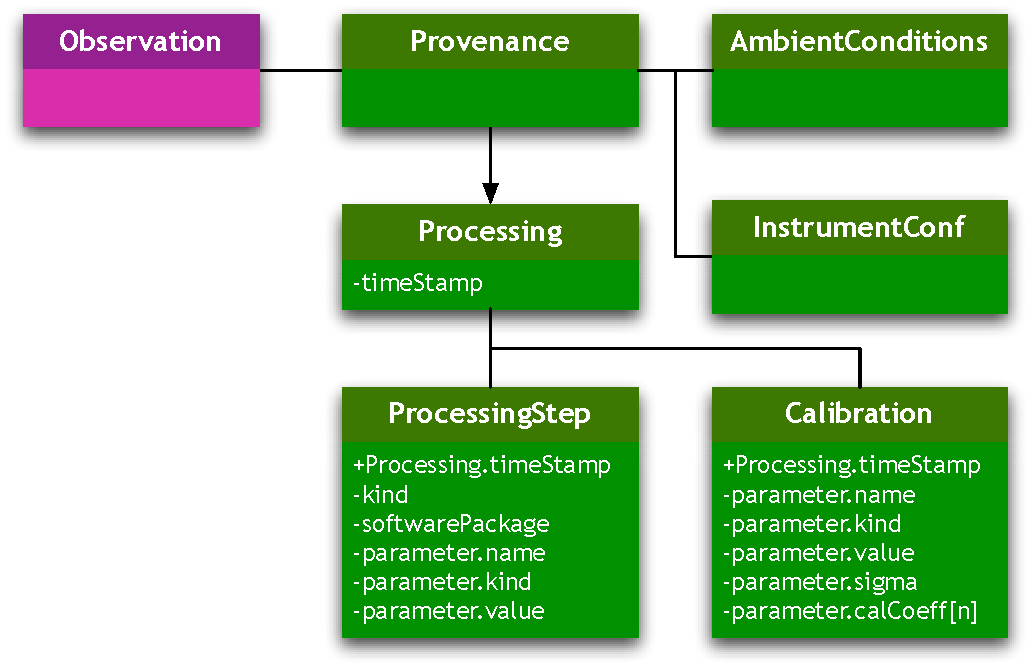
\includegraphics[width=0.6\columnwidth]{fig/Provenance-Processing-DM}
		\end{center}
		\caption[Provenance.Processing data model]
			{Provenance.Processing data model.}
		\label{figProvenanceProcessing}
		\end{figure}
		
		\begin{description}
			\item[Processing] It holds information specifying the
			type of processing applied to data before archival.
			This includes pseudo-observational techniques such as
			position switching or frequency switching, as well as
			the type of data averaging, data weighting, et cetera.
			Table \ref{tabProvenanceProcessingStep} provides
			minimal initial metadata, using arrays of parameter
			keywords for extensibility at the expense of
			complexity.
			
			 \item[Calibration] It is a subclass of Processing,
			where the type of processing is dataCalibration. In
			this class there are additional attributes to specify
			the type of calibration, and the axes to where this
			calibration will be applied. Table
			\ref{tabProvenanceCalibration} provides minimal initial
			metadata, using arrays of parameter keywords for
			extensibility at the expense of complexity.
		\end{description}
		
		 We still have to develop a calibration and/or pointing
		model; maybe based upon IRAM-Multi-Beam-FITS, or GBT FITS
		calibration tables.

		\begin{table}
		\begin{minipage}{\linewidth}
		\caption[Processing Step]{Processing Step metadata.}
		\begin{smallertabular}{p{2.75 cm}p{1.5cm}p{2.25cm}p{4.75cm}}
				& \textbf{FITS} & & \\ \textbf{Attribute} & \textbf{Keyword} &
		        \textbf{UCD} & \textbf{Description}\\ \midrule timestamp &
		        \texttt{DATE-RED} & \texttt{obs.param; time.epoch} & Timestamp
		        for the processing step being performed.\\ \addlinespace type &
		        \texttt{assign} & \texttt{obs.param; meta.code} & Type of
		        processing applied to source data; comes from a controlled
		        vocabulary: \texttt{un\-proc\-essed},
		        \texttt{noise\-Weight\-ed\-Av\-er\-age},
		        \texttt{non\-Weight\-ed\-Av\-er\-age}.\\ \addlinespace
		        software\-Package & \texttt{assign} & \texttt{meta.software;
		        meta.id} & Software package used for data processing; should
		        come from a controlled vocabulary: \texttt{CLASS},
		        \texttt{AIPS}, \texttt{AIPS++}, \texttt{CASA}, \texttt{MOPSIC},
		        \texttt{GILDAS}, \texttt{MIRA}, \texttt{MIR}, \texttt{other}.
		        In the case of \texttt{other}, the actual package that was used
		        should be added as a parameter, with parameter.name as
		        \texttt{software\-Package} and the parameter.value as the
		        package name. \\ \addlinespace parameter[n].name & \texttt{assign} &
		        \texttt{obs.param; meta.code} & Additional processing parameter
		        name, whose value will be in parameter.value; eventually, we
		        will have a controlled list of possible parameter.name
		        values.\\ \addlinespace parameter[n].type & \texttt{assign} &
		        \texttt{obs.param; meta.code} & From a controlled vocabulary:
		        \texttt{integer}, \texttt{float}, \texttt{string}, et cetera.
				At least all
		        of FITS data types should be present.\\ \addlinespace
		        parameter[n].value & \texttt{assign} &
		        \texttt{obs.param}\footnote{The final UCD to mark
		        parameter[n].value will be calculated when writing the VOTable,
		        as it depends on parameter.type; it will be \texttt{obs.param;
		        meta.number} most of the time, but it could be
		        \texttt{obs.param; meta.name} or \texttt{obs.param; meta.code},
		        depending on the context.} & Value for the parameter indicated
		        by parameter.name.\\ \addlinespace
		\end{smallertabular}
		\label{tabProvenanceProcessingStep}
		\end{minipage}
		\end{table}

		\begin{table}
		\begin{minipage}{\linewidth}
		\caption[Calibration metadata]
		{
			Calibration metadata\footnote{It is mandatory that at least one
			\texttt{[parameter.name, parameter.type, parameter.value]}
			triplet appears, with \texttt{fluxScale} as parameter.name, and
			one of \texttt{antennaTemperature},
			\texttt{mbBrightnessTemperature}, or \texttt{S\_nu} as the
			parameter.value, with a parameter.type of \texttt{string}.}.
		}
		\begin{smallertabular}{p{3.15 cm}p{1.5cm}p{2.0cm}p{4.60cm}}
				& \textbf{FITS} & & \\ \textbf{Attribute} & \textbf{Keyword} &
		        \textbf{UCD} & \textbf{Description}\\ \midrule timestamp &
		        \texttt{DATE-RED} & \texttt{obs.param; time.epoch} & Timestamp
		        for the calibration step being performed.\\ \addlinespace
		        parameter.name & \texttt{assign} & \texttt{obs.calib;
		        obs.param; meta.id} & Keyword defining the parameter that we
		        will characterise with the remaining attributes.\\
		        \addlinespace parameter.type & \texttt{assign} &
		        \texttt{obs.calib; obs.param; meta.code} & Type of calibration
		        parameter used, from a controlled vocabulary:
		        \texttt{additive}, \texttt{fac\-tor}, \texttt{pol\-y\-no\-mi\-al},
		        \texttt{ex\-po\-nen\-tial}, \texttt{log\-a\-rith\-mic}.\\
		        \addlinespace parameter.value & \texttt{assign} &
		        \texttt{obs.calib; obs.param; meta.number} & Value for the main
		        calibration parameter, where parameter.type is not
		        \texttt{polynomial}.\\ \addlinespace parameter.sigma &
		        \texttt{assign} & \texttt{obs.calib; obs.param; meta.number} &
		        Value of sigma, for \texttt{exponential} calibrations.\\
		        \addlinespace parameter.calCoeff.[n] & \texttt{assign} &
		        \texttt{obs.calib; obs.param; meta.number} & $\mathrm{n^{th}}$
		        degree coefficient for a \texttt{polynomial} calibration
		        parameter; polynomial degree is derived from the maximum n.\\
		        \addlinespace
		\end{smallertabular}
		\label{tabProvenanceCalibration}
		\end{minipage}
		\end{table}
		
		
	% section processing_provenance (end)
	
	
	\section{Conclusions} % (fold)
	\label{sec:data_provenance_conclusions}
		
		With this chapter we have finished our task of defining
		the modules suggested for the ObsDM, with the objective
		of being able to create a complete data model which
		could be used as a blueprint for archive development.
		
		The Provenance data model is the most instrument dependant
		of the RADAMS models, but of the three sub-models, only
		the Instrument part is strictly specific to radio astronomy.
		This is a strength, however, as the Environment and 
		Processing can be considered part of the atmosphere, and
		part of the workflow, and they are equally needed for all
		kinds of observations. By having the Instrument specific
		signature encapsulated in the Provenance.Instrument
		sub-model, it can be replaced by different
		Provenance.Instrument descriptions, 
		meaningful for the different data analysis packages, which
		are the ones that need the instrument-specific
		information.
	
		
		
	% section data_provenance_conclusions (end)
	
% chapter radams_data_provenance (end)